\clearpage
\section{Elecció de paràmetres $S/C$ i $\Psi$}
Es parteix del coneixement que el treball específic que ha de subministrar el nostre motor és $\tau_{23} = 300000 J/kg$.\\

A partir de motors similars, s'aprecia que les solucions per compressors estan entre 7, 8, 9 i 10 graons. Per tant, per cada un dels 4 casos es pot trobar el valor que es tindria de solidesa i el coeficient de flux del gràfic de $\tau_{esc}$. S'escollirà el cas que tingui un major rendiment per escaló de tots els possibles. \\

Primer de tot es necessari saber el treball específic que ha de realitzar cada etapa de compressió segons el numero total d'etapes. Es calcula com $\tau_{esc}=\tau_{23}/N$ on $N$ és el número d'etapes de compressió.

\begin{longtable}[H]{C{1.5cm} C{2.5cm}}
	\toprule[2pt]
	\textbf{N} &  \textbf{$\tau_{esc} \quad [J/kg]$} \\ \bottomrule[2pt]
	7 & $4.29\mathrm{x}10^4$\\ \midrule
	8 & $3.75\mathrm{x}10^4$\\ \midrule
	9 & $3.33\mathrm{x}10^4$\\ \midrule
	10&$3.00\mathrm{x}10^4$
	\\ \bottomrule[2pt]
	\caption{Treball específic segons etapes de compressió}
	\label{valorsI}
\end{longtable}

Després, es superposen (Figura \ref{TAUS}) els resultats obtinguts per cada escaló segons nombre d'etapes amb els valors de $\tau$ inicialment calculats per diferents $S/C$ i $\Psi$.\\
\begin{figure}[H]
	\centering
	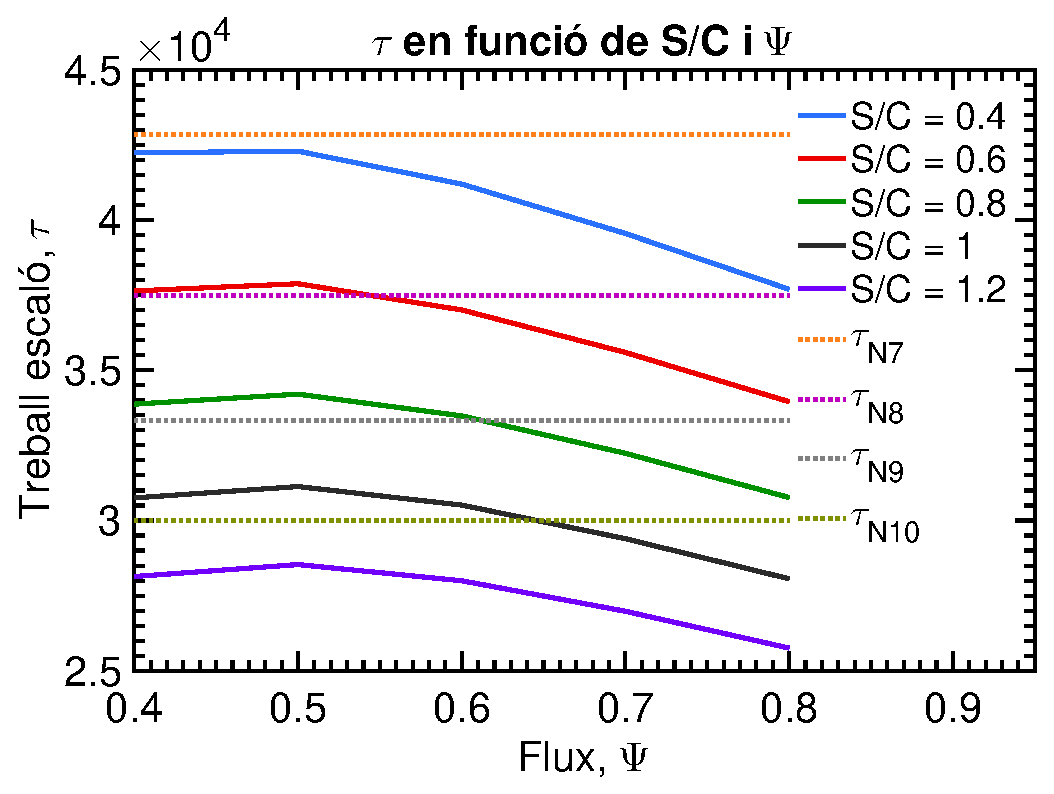
\includegraphics[width=0.8\textwidth]{./code/figures/parametres/TAUSesg.eps}
	\caption{Valors de $\tau$ en funció de $S/C$ i $\Psi$.}
	\label{TAUS}
\end{figure}
\clearpage

Es busca l'intersecció dels treballs específics calculats per a cada etapa amb els treballs d'escaló calculats per per diferents valors de $S/C$ i $\Psi$.

El resultat, permet veure quin paràmetre $S/C$ es el millor per a cada punt d'intersecció, però per saber el flux ($\Psi$) caldrà interpolar entre els dos punts més propers a l'intersecció.\\

S'han interpolat els valors del flux ($\Psi$) linealment a partir de dos punts d'informació propers a l'intersecció, $(x_a,y_a)$ i $(x_b,y_b)$, per obtenir un tercer punt interpolat $(x,y)$ segons,
\begin{equation}
	y = y_a + (x-x_a)\frac{(y_b-y_a)}{(x_b-x_a)}
\end{equation}
per aquest cas particular,
\begin{equation}
\Psi_N = \Psi_a + (\tau_{N}-\tau_a)\frac{(\Psi_b-\Psi_a)}{(\tau_b-\tau_a)}
\end{equation}

Aquesta aproximació lineal, és vàlida ja que es treballa en un interval petit entre les dues dades conegudes. Finalment, els resultats obtinguts apareixen agrupats a la Taula \ref{paramIni}.

\begin{longtable}[H]{C{1.5cm} C{1.5cm} C{1.5cm}}
	\toprule[2pt]
	\textbf{N} &  \textbf{$S/C$}  & \textbf{$\Psi$}\\ \bottomrule[2pt]
	7 & -- & --\\ \midrule
	8 & 0.6 &0.5437\\ \midrule
	9 & 0.8 &0.6121\\ \midrule
	10 & 1 &0.6455
	\\ \bottomrule[2pt]
	\caption{Paràmetres escollits inicialment}
	\label{paramIni}
\end{longtable}

\subsection{Selecció del cas amb major rendiment}
\begin{figure}[H]
	\centering
	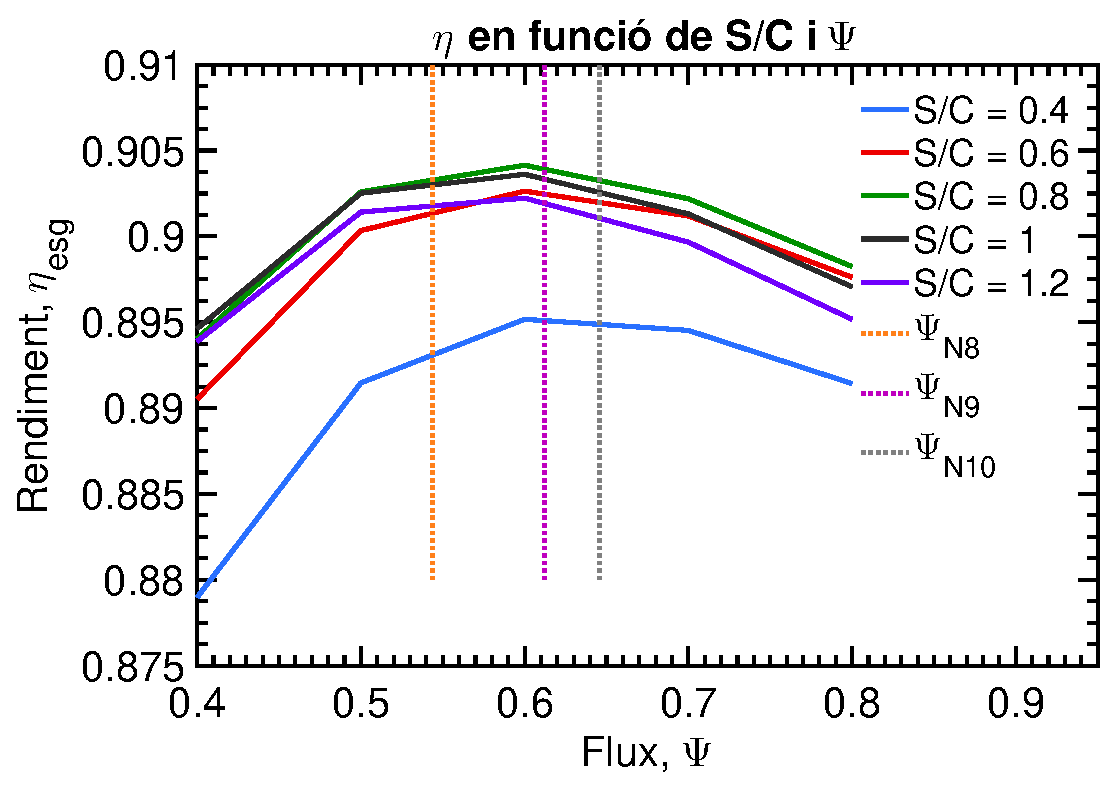
\includegraphics[width=0.8\textwidth]{./code/figures/parametres/FLUXs}
	\caption{Valors de $\eta$ en funció de $S/C$ i $\Psi$.}
	\label{FLUXs}
\end{figure}
Un cop se saben els paràmetres $S/C$ i $\Psi$, per trobar els rendiments associats, se superposen els valors de $\eta$ en funció de $S/C$ i $\Psi$ calculats amb anterioritat amb els valors de $\Psi$ de la Taula \ref{paramIni}. Aquest procés està il·lustrat a la Figura \ref{FLUXs}.\\

A l'igual que el primer cas, ara s'interpola el valor de $\eta$ entre els dos punts més pròxims a l'intersecció. Obtenint-se els resultats de la Taula \ref{paramEta}
\begin{longtable}[H]{C{1.5cm} C{1.5cm} C{1.5cm} C{1.5cm}}
	\toprule[2pt]
	\textbf{N} &  \textbf{$S/C$}  & \textbf{$\Psi$}& \textbf{$\eta_{esc}$}\\ \bottomrule[2pt]
	7 & -- & -- & --\\ \midrule
	8 & 0.6 &0.5437 & 0.9013 \\ \midrule
	9 & 0.8 &0.6121 & 0.9039\\ \midrule
	10 & 1 &0.6455& 0.9026
	\\ \bottomrule[2pt]
	\caption{Paràmetres escollits inicialment, més $\eta_{esc}$}
	\label{paramEta}
\end{longtable}

La primera impressió, es de que el compressor de 9 etapes, té el millor rendiment. Tot i això, és necessari calcular el rendiment total del compressor per veure si és realment així, ja que tots els rendiments tenen valors molt similars entre si.\\

A partir de l'equació \ref{eq23} es pot calcular el rendiment total del compressor. Per fer-ho, com en els anteriors casos, es necessari interpolar els valors de $C_D$ i $C_{Li}$, seguint el mateix principi.

\begin{equation}
	\eta_{23} = 1-N\frac{C_D}{C_{Li}}\Big(2\Psi+\frac{1}{2\Psi}\Big)
	\label{eq23}
\end{equation}

\begin{longtable}[H]{C{1.5cm} C{1.5cm} C{1.5cm} C{1.5cm}}
	\toprule[2pt]
	\textbf{N} &  \textbf{$S/C$}  & \textbf{$\Psi$}& \textbf{$\eta_{23}$}\\ \bottomrule[2pt]
	7 & -- & -- & --\\ \midrule
	8 & 0.6 &0.5437 & 0.2142 \\ \midrule
	9 & 0.8 &0.6121 & 0.1360\\ \midrule
	10 & 1 &0.6455& 0.0278
	\\ \bottomrule[2pt]
	\caption{Paràmetres escollits inicialment, més $\eta_{23}$}
	\label{paramEta23}
\end{longtable}
Els resultats obtinguts són molt interessants, ja que mostren que el compressor més eficient és el de 8 etapes, per tant, els paràmetres escollits són:
\begin{longtable}[H]{C{1.5cm} C{1.5cm} C{1.5cm}}
	\toprule[2pt]
	\textbf{N} &  \textbf{$S/C$}  & \textbf{$\Psi$}\\ \bottomrule[2pt]
	8 & 0.6 &0.5437\\ \bottomrule[2pt]
	\caption{Paràmetres escollits}
	\label{param}
\end{longtable}

Finalment, es verifica que el rang de velocitat axial estigui entre 150m/s i 180m/s com s'ha comentat anteriorment a l'informe. També es verifica que la velocitat axial no superi els 320m/s per tal de no comprometre estructuralment els àleps. A la Taula \ref{paramExtra} es pot comprovar que els valors estan dins dels rangs vàlids.\\
\\

\begin{longtable}[H]{C{1.5cm} C{1.5cm} C{1.5cm} C{1.5cm} C{1.5cm} C{1.5cm}}
	\toprule[2pt]
	\textbf{$V_z [m/s]$} &  \textbf{$u[m/s]$}  & \textbf{$C_L$}& \textbf{$C_D$}& \textbf{$\eta_{esc}$}& \textbf{$\eta_{23}$}\\ \bottomrule[2pt]
		160.73 & 290.24 &0.6990&0.0346&0.9013&0.2142\\ \bottomrule[2pt]
		\caption{Paràmetres interpolats per $N = 8$, $S/C=0.6$ i $\Psi=0.5437$ }
		\label{paramExtra}
	\end{longtable}